\pagestyle{fancy}
\section{Introducción}

Airon Tools es una empresa mexicana con más de una década de experiencia en la comercialización de herramientas industriales para el sector mecánico y automotriz. Actualmente enfrenta desafíos operativos derivados del uso de procesos manuales y herramientas no integradas para la gestión interna y atención a clientes.

La gestión de servicios técnicos, inventario y comunicación interna se realiza mediante hojas de cálculo y formatos físicos, lo que ha derivado en dificultades para la trazabilidad, errores en registros, pérdida de datos y una experiencia limitada para el cliente. Estas deficiencias afectan la eficiencia operativa y competitividad frente a empresas del sector que ya operan con sistemas digitales.

El objetivo del proyecto es desarrollar una plataforma integral que centralice la información, mejore la trazabilidad de servicios, optimice el control de inventario y facilite la comunicación entre áreas operativas. El sistema se construirá bajo una arquitectura escalable que garantice su adaptabilidad y crecimiento.

Como beneficio, se espera una mejora en los tiempos de respuesta, administración más eficiente de recursos, atención al cliente más ágil y un fortalecimiento de la capacidad competitiva. El presente proyecto se enmarca dentro de la modalidad de experiencia profesional, respondiendo a una necesidad real detectada en la operación de la empresa.

\section{Justificación}

La propuesta surge de una necesidad concreta identificada en la operación diaria de Airon Tools. La falta de un sistema de gestión digitalizado ha derivado en atención deficiente al cliente, escasa trazabilidad de servicios técnicos y desorganización en el control de inventario. Los registros actuales se realizan mediante formatos físicos o archivos aislados, generando errores, pérdida de información y demoras que impactan la eficiencia y la imagen profesional de la empresa.

La implementación de un sistema de gestión integral permitirá centralizar la información relacionada con empleados, clientes, servicios y productos. La automatización de notificaciones y digitalización de procesos facilitarán la trazabilidad del flujo de trabajo y establecerán una comunicación más eficiente con los clientes. Además, la optimización del control de inventario mediante reportes automáticos reducirá errores y facilitará la toma de decisiones basadas en datos reales.

Esta propuesta tecnológica contribuirá a mejorar la productividad interna y elevar la calidad del servicio ofrecido, posicionando a Airon Tools como una empresa moderna y eficiente en un mercado altamente competitivo.

\section{Objetivo general}
Diseñar un sistema digital de gestión empresarial para Airon Tools que automatice y centralice los procesos internos de atención al cliente, servicios técnicos, control de inventario y comunicación organizacional, con el fin de mejorar la eficiencia operativa, la trazabilidad de los servicios y la calidad del servicio ofrecido.

\section{Objetivos específicos}
\begin{enumerate}
    \item Implementar un módulo de gestión de Empleados que permita registrar, editar y organizar al personal de Airon Tools, asignando roles y permisos según sus funciones operativas.

    \item Desarrollar un módulo de clientes para registrar, consultar y actualizar información de clientes particulares y corporativos, incluyendo su historial de atención.

    \item Automatizar el proceso de servicios técnicos mediante un módulo que registre cada solicitud, seguimiento por etapas y finalización del servicio, con notificaciones automáticas integradas.

    \item Crear un módulo de inventario que permita gestionar productos y herramientas mediante funciones de alta, consulta, edición y eliminación, manteniendo un catálogo actualizado.
\end{enumerate}


\section{Trabajos relacionados}

A continuación se presentan seis trabajos que abordan problemáticas similares a las identificadas en el presente proyecto. Se analiza su propósito, contexto, solución implementada y resultados obtenidos, con el fin de establecer un marco de referencia que oriente el diseño del sistema propuesto para Airon Tools.

\subsection{Elaboración de un sistema de gestión por procesos aplicado a una empresa dedicada a la distribución y comercialización de productos de ferretería y materiales de construcción \cite{Vargas2018}.}

Proyecto integrador desarrollado en la Escuela Superior Politécnica del Litoral, Ecuador, que mejoró la eficiencia operativa de una empresa ferretera mediante la estandarización de procesos. Se implementó un sistema de gestión documentando operaciones clave y utilizando herramientas como análisis FODA y KPIs, resultando en una propuesta organizacional para optimizar la toma de decisiones.

\subsection{Desarrollo de un sistema de gestión por procesos para empresas de servicios de ingeniería y construcción orientadas a la industria \cite{Munoz2018}.}

Tesis de maestría que mejoró la eficiencia organizacional de CDM S.A. mediante un sistema de gestión basado en la norma ISO 9001:2015. La propuesta integró procesos estratégicos y operativos utilizando mapas de procesos y mecanismos de mejora continua, resultando en un modelo estructurado para la documentación y control de operaciones.

\subsection{Diseño de un sistema de gestión basado en procesos \cite{Jacome2016}.}

Tesis de maestría de la Universidad Andina Simón Bolívar que propuso un sistema de gestión para una empresa tecnológica con baja eficiencia administrativa. La solución, basada en normas ISO y análisis de procesos, resultó en un modelo que fortaleció la claridad organizacional y facilitó la toma de decisiones estratégicas.

\subsection{Proceso Administrativo y Gestión Empresarial en COPROABAS, Jinotega \cite{Flores15}.}

Tesis de maestría que mejoró el desempeño organizacional de la cooperativa COPROABAS mediante el fortalecimiento de su gestión administrativa. La investigación identificó deficiencias estructurales y propuso mejoras para optimizar la planificación y control dentro de la cooperativa.

\subsection{Principales causas del fracaso en la implementación de un ERP: el caso de una PyME en México \cite{Delgado2015}.}

Tesis de maestría de la UNAM que identificó las causas del fracaso en la implementación de sistemas ERP en PyMEs mexicanas. Mediante el método Delphi, se detectaron deficiencias en capacitación y planeación estratégica, concluyendo con recomendaciones para mejorar la ejecución de proyectos ERP.

\subsection{Planeación Estratégica y Nuevos Proyectos en Empresa Propia \cite{Patino19}.}

Proyecto terminal de la Universidad ICESI que consolidó la planeación estratégica de una empresa apícola en fase inicial. Mediante análisis FODA y modelo Canvas, se definieron objetivos estratégicos y proyecciones financieras para orientar su crecimiento competitivo.

% NOTA: Actualizar también la tabla de comparación si es necesario.

\begin{longtable}{m{.05\paperwidth} *{2}{m{.33\paperwidth}} @{}}
	\caption{Comparación cualitativa de los trabajos relacionados con el proyecto.}
	\label{table:trabajosRelacionados}\\
	\hline
	\textbf{Ref.} & \textbf{Similitudes} & \textbf{Diferencias} \\
	\hline
	\endfirsthead
	
	\multicolumn{3}{c}{\textbf{Continuación de la Tabla \ref{table:trabajosRelacionados}}} \\
	\hline
	\textbf{Ref.} & \textbf{Similitudes} & \textbf{Diferencias} \\
	\hline
	\endhead
	\hline
	\endlastfoot

	\cite{Vargas2018} &
	\begin{itemize}
	  \item Gestión por procesos como enfoque estructural
	  \item Mejora de eficiencia operativa y toma de decisiones
	  \item Problemáticas de control y duplicidad de funciones
	\end{itemize} &
	\begin{itemize}
	  \item Vargas usa herramientas formales (FODA, KPIs); \hl{este proyecto} se basa en diagnóstico interno
	  \item Sin desarrollo tecnológico; \hl{este sistema} incluye plataforma completa con backend y frontend
	  \item Enfoque contable; \hl{este sistema} abarca trazabilidad digital y automatización
	\end{itemize} \\	
\midrule

\cite{Munoz2018} &
\begin{itemize}
  \item Sistema centrado en procesos estratégicos y de soporte
  \item Solución basada en deficiencias internas
  \item Mejora de estructura organizacional
\end{itemize} &
\begin{itemize}
  \item Sin sistema digital; \hl{este proyecto} implementa plataforma con NestJS, React y MongoDB
  \item Enfoque documental; \hl{este sistema} automatiza procesos y permite trazabilidad
  \item \hl{Esta solución} está en la nube con arquitectura multitenant
\end{itemize} \\

\cite{Jacome2016} &
\begin{itemize}
  \item Sistemas de gestión orientados a procesos
  \item Estructuración de operaciones críticas
  \item Control y optimización de procesos clave
\end{itemize} &
\begin{itemize}
  \item Solución conceptual; \hl{este proyecto} desarrolla plataforma funcional
  \item \hl{Este sistema} integra comunicación en tiempo real y automatización
  \item Orientado al sector industrial de herramientas
\end{itemize} \\

\cite{Flores15} &
\begin{itemize}
  \item Análisis de fallas organizacionales
  \item Fortalecimiento de gestión empresarial
  \item Soluciones a problemas de gestión
\end{itemize} &
\begin{itemize}
  \item Enfoque cualitativo tradicional; \hl{este proyecto} desarrolla solución digital
  \item \hl{Este sistema} usa tecnologías modernas con automatización
  \item Incluye comunicación en tiempo real y soporte multitenant
\end{itemize} \\

\cite{Delgado2015} &
\begin{itemize}
  \item Problemáticas de eficiencia organizacional
  \item Importancia de gestión de procesos
  \item Relevancia de estructura organizacional
\end{itemize} &
\begin{itemize}
  \item Análisis de fracasos en ERPs; \hl{este proyecto} desarrolla solución funcional
  \item Enfoque teórico; \hl{este sistema} es aplicado en empresa real
  \item \hl{Esta solución} automatiza procesos y permite trazabilidad digital
\end{itemize} \\

\cite{Patino19} &
\begin{itemize}
  \item Necesidad empresarial en organizaciones jóvenes
  \item Fortalecimiento de estructura interna
  \item Consolidación de procesos para crecimiento
\end{itemize} &
\begin{itemize}
  \item Enfoque en planeación estratégica; \hl{este proyecto} se basa en necesidades internas
  \item Sin soluciones tecnológicas; \hl{esta propuesta} incluye sistema completo
  \item \hl{Este sistema} incorpora automatización y soporte multitenant
\end{itemize} \\
\bottomrule
\end{longtable}

	

\section{Descripción técnica}

El sistema propuesto es una aplicación web de gestión empresarial compuesta por módulos funcionales que automatizan y centralizan los procesos clave de Airon Tools. Está orientado a mejorar la atención al cliente, administración de servicios técnicos, control de productos y coordinación interna, bajo una arquitectura escalable.

\subsection*{Arquitectura general del sistema}

El sistema sigue una arquitectura modular cliente-servidor con backend y frontend desacoplados mediante APIs RESTful, permitiendo flexibilidad e integración futura.

La Figura~\ref{fig:arquitectura} muestra una vista general de la arquitectura del sistema con sus principales componentes.

\begin{figure}[H]
	\centering
	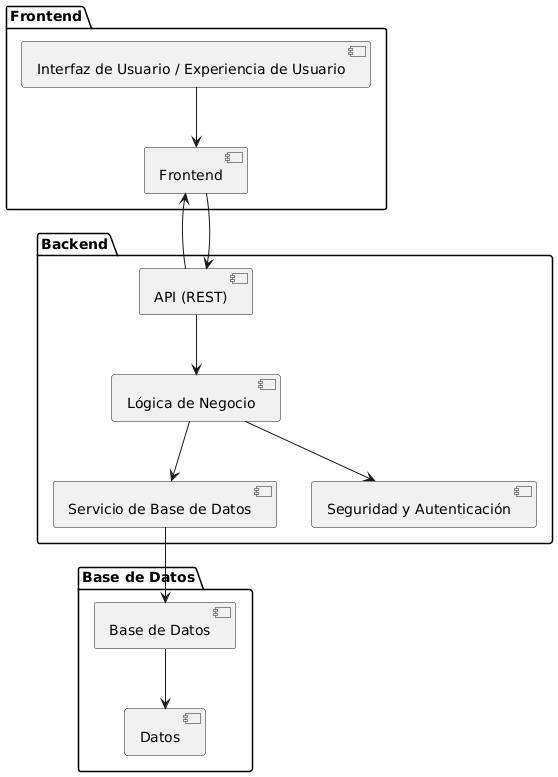
\includegraphics[width=0.6\textwidth]{sistema.png}
	\caption{Arquitectura general del sistema propuesto para Airon Tools.}
	\label{fig:arquitectura}
\end{figure}

\subsection*{Módulos del sistema}

\begin{itemize}
    \item \textbf{Empleados y roles:} Registro de empleados, roles y permisos de acceso con autenticación.
    \item \textbf{Clientes:} Registro de clientes con historial de servicios e integración de notificaciones.
    \item \textbf{Servicios técnicos:} Automatización del flujo de atención con notificaciones automáticas.
    \item \textbf{Productos:} Gestión de productos con información detallada e integración con servicios.
    \item \textbf{Notificaciones:} Sistema de notificaciones por correo y comunicación interna en tiempo real.
\end{itemize}

\section{Especificación técnica}

El sistema será accesible mediante una aplicación web con arquitectura modular, integrando:

\begin{itemize}
	\item \textbf{Backend:} NestJS con TypeScript, arquitectura modular con controladores y servicios.
	\item \textbf{Frontend:} React.js con TypeScript, implementando Clean Architecture.
	\item \textbf{Base de datos:} MongoDB con soporte multitenant.
	\item \textbf{Interfaz:} HTML5, CSS3, Figma y TailwindCSS.
	\item \textbf{Comunicación:} WebSockets y SMTP.
	\item \textbf{DevOps:} Git, GitHub Actions, Docker y AWS.
\end{itemize}

\subsection*{Alcance funcional}

El proyecto implementará:
\begin{itemize}
	\item Gestión de empleados y autenticación
	\item Registro y administración de clientes
	\item Flujo de servicios técnicos
	\item Catálogo digital de productos
	\item Sistema de notificaciones
	\item Respaldo y reportes
	\item Soporte multitenant
\end{itemize}

\subsection*{Criterios de finalización}

El sistema se considerará funcional cuando:
\begin{itemize}
	\item Los módulos estén implementados y probados
	\item Los casos de uso estén validados
	\item El sistema esté desplegado en pruebas
	\item Se entregue la documentación técnica
	\item Se incluya el código fuente en los apéndices
\end{itemize}

	Cada módulo será considerado finalizado cuando cumpla con los casos de uso definidos, haya sido probado funcionalmente y esté debidamente documentado. Además, el sistema deberá encontrarse desplegado en un entorno de pruebas funcional para su demostración.
	
	\vspace{0.5cm}
	
	%Este texto SÍ debe incluirse para que la propuesta pueda ser aceptada.
	Al concluir el proyecto de integración se entregará a la Coordinación de Estudios de Ingeniería en Computación una carpeta digital que incluirá el reporte final del proyecto en un archivo PDF (sin restricciones)\footnote{Debe poder visualizarse sin solicitar contraseña}, el código fuente del proyecto en un archivo comprimido (sin restricciones)\footnote{Debe poder descomprimirse sin solicitar contraseña}. Además, la sección de apéndices del reporte final contendrá al menos un listado del código fuente desarrollado.


	\section{Calendario de actividades}

Las actividades a realizar durante el Trimestre 2025-Invierno en la UEA Proyecto de Integración de Ingeniería en Computación I (clave 1100113), con un valor de 18 créditos y una duración total de 198 horas, se presentan en la Tabla~\ref{table:calendarioActividades}.

\begin{longtable}{p{0.05\textwidth} p{0.4\textwidth} p{0.1\textwidth} p{0.35\textwidth}}
	\caption{Listado de actividades a realizar durante el Trimestre 2025-Invierno.}
  	\label{table:calendarioActividades}\\
	\toprule
	\textbf{No.} & \textbf{Actividad} & \textbf{Horas} & \textbf{Entregable} \\
	\hline
	\endfirsthead

	\multicolumn{4}{c}{\textbf{Continuación de la Tabla \ref{table:calendarioActividades}}}\\
	\hline
	\textbf{No.} & \textbf{Actividad} & \textbf{Horas} & \textbf{Entregable} \\
	\hline
	\endhead

	\hline
	\endlastfoot

	1 & Levantamiento de requerimientos y análisis del sistema actual en Airon Tools. & 20 & Documento de requerimientos \\
	\midrule

	2 & Diseño de arquitectura del sistema y definición de módulos. & 20 & Diagramas de arquitectura y diseño técnico \\
	\midrule

	3 & Desarrollo del módulo de autenticación y gestión de usuarios. & 25 & Módulo funcional con control de acceso y roles \\
	\midrule

	4 & Desarrollo del módulo de gestión de clientes. & 20 & Registro, historial y vista de clientes implementados \\
	\midrule

	5 & Desarrollo del módulo de servicios técnicos (flujo completo). & 25 & Módulo de flujo de servicio técnico automatizado \\
	\midrule

	6 & Desarrollo del módulo de inventario. & 20 & Registro, movimientos y alertas de inventario \\
	\midrule

	7 & Implementación de sistema de notificaciones y comunicación interna. & 20 & Notificaciones por correo, alertas internas y tareas asignadas \\
	\midrule

	8 & Pruebas funcionales e integración de los módulos. & 20 & Reporte de pruebas, casos de uso validados \\
	\midrule

	9 & Despliegue en entorno de pruebas y revisión técnica. & 15 & Sistema desplegado en servidor y documentación preliminar \\
	\midrule

	10 & Documentación técnica y elaboración de manual de usuario. & 13 & Manual de usuario, guía de instalación y documentación del sistema \\
	\bottomrule
\end{longtable}

\footnotetext{La planeación cubre el análisis, diseño, desarrollo, pruebas, despliegue y documentación del sistema, abarcando las 198 horas correspondientes a la UEA mencionada.}




\section{Factibilidad técnica y operativa}

\subsection{Factibilidad técnica}

El proyecto de desarrollo del sistema de gestión empresarial para Airon Tools es técnicamente viable, ya que el responsable del desarrollo cuenta con los conocimientos y habilidades necesarios para implementar los módulos definidos en el tiempo estipulado. Entre las competencias destacadas se encuentran:

\begin{itemize}
	\item Conocimientos avanzados en desarrollo web fullstack utilizando tecnologías como React.js, TypeScript y NestJS.
	\item Experiencia en diseño e implementación de arquitecturas modulares y sistemas empresariales.
	\item Habilidad en pruebas, documentación técnica y despliegue de sistemas.
\end{itemize}

Los recursos disponibles para el desarrollo y pruebas del sistema son los siguientes:

\begin{itemize}
	\item Equipos de cómputo con procesadores Intel Core i7, 16 GB de RAM y almacenamiento SSD.
	\item Acceso a entornos locales y servidores remotos para pruebas y despliegue del sistema.
	\item Conectividad de red estable para realizar pruebas multiusuario y simulaciones reales.
\end{itemize}

Las herramientas que se utilizarán durante el desarrollo incluyen:

\begin{itemize}
	\item \textbf{Frontend:} React.js con TypeScript, Figma para prototipado, y TalwindCSS para diseño de interfaz.
	\item \textbf{Backend:} NestJS con Node.js y MongoDB como base de datos.
	\item \textbf{Control de versiones:} Git y GitHub.
	\item \textbf{Contenedores y despliegue:} Docker, GitHub Actions para integración y entrega continua.
\end{itemize}

No se requieren recursos físicos adicionales ni licencias de software especiales, ya que todas las herramientas son de uso libre o ya están disponibles.

\subsection{Factibilidad operativa}

El sistema propuesto presenta una alta factibilidad operativa dentro de la empresa Airon Tools, por las siguientes razones:

\begin{itemize}
	\item \textbf{Adaptabilidad a los procesos actuales:} El sistema está alineado con los flujos de trabajo reales de la empresa, por lo que su adopción no requerirá una reestructuración significativa.
	
	\item \textbf{Aceptación organizacional:} El proyecto cuenta con el respaldo directo del jefe de área, el Ing. Víctor Benjamín Aguilar Orocio, responsable de la implementación en la empresa.
	
	\item \textbf{Capacitación del personal:} Se prevé una estrategia de introducción y formación progresiva, asegurando que los empleados comprendan y utilicen el sistema eficazmente.
	
	\item \textbf{Facilidad de uso y soporte:} La interfaz estará diseñada con criterios de usabilidad, y el sistema incluirá funciones de ayuda y comunicación interna que facilitarán su soporte continuo.
	
	\item \textbf{Extensibilidad y mantenimiento:} Gracias a su arquitectura modular, el sistema podrá adaptarse a futuras necesidades o integrarse con nuevas tecnologías sin comprometer su estabilidad.
\end{itemize}


\vspace{0.5cm}\vspace{0.5cm}
\section{Estimación de costos}

La presente sección muestra una estimación comercial del capital necesario para el desarrollo del sistema de gestión empresarial propuesto, considerando tanto los recursos técnicos como el valor del trabajo intelectual involucrado. Se han incluido costos asociados a infraestructura, herramientas, servicios y personal. Esta estimación representa una aproximación realista en caso de que el proyecto se desee escalar o comercializar.

La estimación de costos del proyecto se presenta en la Tabla~\ref{table:tablaCostos}.

\begin{longtable}{m{6.5cm} m{4.5cm} m{4cm}}
	\caption{Estimación de costos del proyecto.}
  	\label{table:tablaCostos}\\
  	\toprule
	\textbf{Descripción} & \textbf{Costo unitario (MXN)} & \textbf{Costo total (MXN)} \\
	\hline
	\endfirsthead

	\multicolumn{3}{c}{\textbf{Continuación de la Tabla \ref{table:tablaCostos}}}\\
	\hline
	\textbf{Descripción} & \textbf{Costo unitario (MXN)} & \textbf{Costo total (MXN)} \\
	\hline
	\endhead

	\hline
	\endlastfoot

Trabajo de desarrollo (fullstack, \hl{3 meses}) & \$9,974.00 $\times$ \hl{3 meses} & \hl{\$29,922.00} \\
\midrule

Desarrollo frontend de apoyo (\hl{3 meses}) & \$8,500.00 $\times$ \hl{3 meses} & \hl{\$25,500.00} \\
\midrule

Computadora personal del desarrollador principal & — & \$12,000.00 \\
\midrule

Computadora personal de la desarrolladora frontend & — & \$12,000.00 \\
\midrule

Servidor local Linux & — & \$8,000.00 \\
\midrule

Cámara digital para registro de productos & — & \$800.00 \\
\midrule

Servicios en la nube (Amazon Web Services, total \hl{3 meses}) & \$\hl{46.15} USD $\approx$ \$\hl{920.59} & \$\hl{920.59} \\
\midrule

Gestión de repositorios (GitHub Teams, plan anual) & \$96.00 USD $\approx$ \$1,915.20 & \$1,915.20 \\
\midrule

\textbf{Costo total estimado} & — & \textbf{\hl{\$91,057.79}} \\
\bottomrule
\end{longtable}

\vspace{0.5cm}

\noindent
\textbf{Nota:} Los montos fueron calculados con base en recibos de nómina, facturas y registros reales generados durante el desarrollo del sistema. Estos datos provienen de pagos y compras efectuados por la empresa, tanto al responsable del proyecto como al personal de apoyo. Los precios de herramientas, servicios y equipos se estimaron conforme a comprobantes de adquisición y consumo. En caso de ser necesario, la empresa puede proporcionar la documentación correspondiente bajo solicitud formal.

\vspace{1cm}